\documentclass[11pt]{article}
\newcommand{\name}{Jingbo Wang}
\usepackage[paper=letterpaper,margin=1in]{geometry}
\usepackage[parfill]{parskip}
\usepackage{amsmath}
\usepackage{fancyvrb}
\usepackage{fancyhdr}
\pagestyle{fancy}
\fancyhf{}
\rhead{\name{}}
\cfoot{Page \thepage}

\newcommand{\problem}[1]{\vspace*{2ex}\textbf{Problem #1 ---} }
\newcommand{\answer}{\emph{Answer: } }

\usepackage{tikz}
\usetikzlibrary{arrows.meta}


\begin{document}
\thispagestyle{empty}

\begin{center}
{\large CS 310}\\
Assignment 304\\
\today
\end{center}

\begin{flushright}
\name{}
\end{flushright}

\problem{1} Given the input 3406, 6672, 4669, 1509, 8446, 9991, 3723,
9381, and 3441, in that order, and the hash function 
$h(x) = 6 - (x \bmod 7)$, draw the resulting hash table. 
State and explain any assumptions you make.

\answer{}

Using hash function $h(x) = 6 - (x \bmod 7)$, we get:
\begin{center}
 $h(3406) = 6 - (3406 \bmod 7) = 6 - 4 = 2$

 $h(6672) = 6 - (6672 \bmod 7) = 6 - 1 = 5$

 $h(4669) = 6 - (4669 \bmod 7) = 6 - 0 = 6$

 $h(1509) = 6 - (1509 \bmod 7) = 6 - 4 = 2$

 $h(8446) = 6 - (8446 \bmod 7) = 6 - 4 = 2$

 $h(9991) = 6 - (9991 \bmod 7) = 6 - 2 = 4$

 $h(3723) = 6 - (3723 \bmod 7) = 6 - 6 = 0$

 $h(9381) = 6 - (9381 \bmod 7) = 6 - 1 = 5$

 $h(3441) = 6 - (3441 \bmod 7) = 6 - 4 = 2$
\end{center}

Here is the hash table:
\begin{center}
% written for clarity, not for efficiency :)
% horizontal coordinates increase left to right
% vertical coordinates increase bottom to top
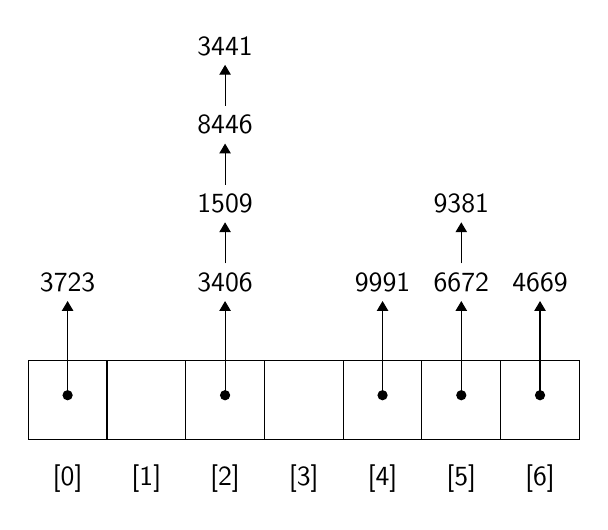
\begin{tikzpicture}[font=\sffamily,scale=0.5]
\draw (0, 0) rectangle (2, 2);
\draw (2, 0) rectangle (4, 2);
\draw (4, 0) rectangle (6, 2);
\draw (6, 0) rectangle (8, 2);
\draw (8, 0) rectangle (10, 2);
\draw (10, 0) rectangle (12, 2);
\draw (12, 0) rectangle (14, 2);
\node (0) at (1, -1) {[0]};
\node (1) at (3, -1) {[1]};
\node (2) at (5, -1) {[2]};
\node (3) at (7, -1) {[3]};
\node (4) at (9, -1) {[4]};
\node (5) at (11, -1) {[5]};
\node (6) at (13, -1) {[6]};
\node (a) at (1, 4) {3723};
\node (b) at (5, 4) {3406};
\node (c) at (5, 6) {1509};
\node (d) at (5, 8) {8446};
\node (e) at (5, 10) {3441};
\node (f) at (9, 4) {9991};
\node (g) at (11, 4) {6672};
\node (h) at (11, 6) {9381};
\node (i) at (13, 4) {4669};
\draw [Circle-Triangle] (1, 1) -- (a);
\draw [Circle-Triangle] (5, 1) -- (b);
\draw [Circle-Triangle] (9, 1) -- (f);
\draw [Circle-Triangle] (11, 1) -- (g);
\draw [Circle-Triangle] (13, 1) -- (i);
\draw [-Triangle] (b) -- (c);
\draw [-Triangle] (c) -- (d);
\draw [-Triangle] (d) -- (e);
\draw [-Triangle] (g) -- (h);
\end{tikzpicture}
\end{center}

\newpage

\problem{2} Assume that conditions indicate a need to rehash 
the hash table from problem 1. Perform a rehash of that hash table, 
and show the hash table that results from the rehashing. 
Explain your process and results.

\answer{}

Because the table gets almost full, and has too much open chaining, 
we need to rehash the original hash table. 

First, we need to allocate a new table of size being more than twice
as big as the current table, and also size is prime number. 
$17 > 2 \times 7$

Therefore, we have new hash function: $h(x) = x \bmod 17$.

Then, we have:
\begin{center}
 $h(3406) = 3406 \bmod 17 = 6$

 $h(6672) = 6672 \bmod 17 = 8$

 $h(4669) = 4669 \bmod 17 = 11$

 $h(1509) = 1509 \bmod 17 = 13$

 $h(8446) = 8446 \bmod 17 = 14$

 $h(9991) = 9991 \bmod 17 = 12$

 $h(3723) = 3723 \bmod 17 = 0$

 $h(9381) = 9381 \bmod 17 = 14$

 $h(3441) = 3441 \bmod 17 = 7$
\end{center}

There is the hash table: 
\begin{center}
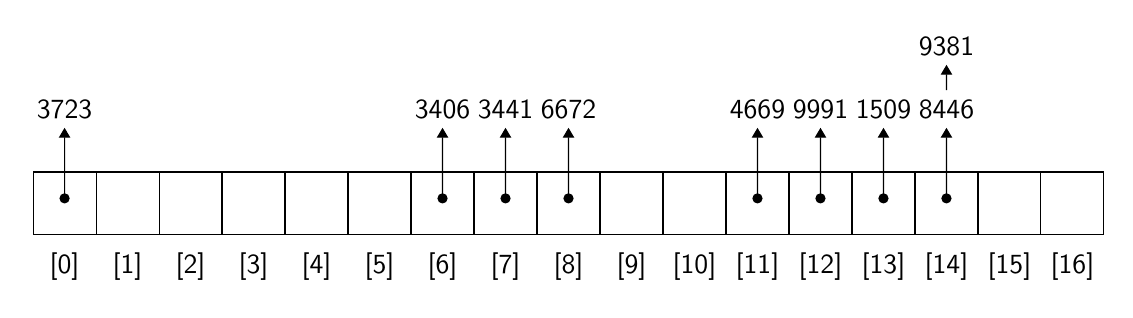
\begin{tikzpicture}[font=\sffamily,scale=0.4]
\draw (0, 0) rectangle (2, 2);
\draw (2, 0) rectangle (4, 2);
\draw (4, 0) rectangle (6, 2);
\draw (6, 0) rectangle (8, 2);
\draw (8, 0) rectangle (10, 2);
\draw (10, 0) rectangle (12, 2);
\draw (12, 0) rectangle (14, 2);
\draw (14, 0) rectangle (16, 2);
\draw (16, 0) rectangle (18, 2);
\draw (18, 0) rectangle (20, 2);
\draw (20, 0) rectangle (22, 2);
\draw (22, 0) rectangle (24, 2);
\draw (24, 0) rectangle (26, 2);
\draw (26, 0) rectangle (28, 2);
\draw (28, 0) rectangle (30, 2);
\draw (30, 0) rectangle (32, 2);
\draw (32, 0) rectangle (34, 2);
\node (0) at (1, -1) {[0]};
\node (1) at (3, -1) {[1]};
\node (2) at (5, -1) {[2]};
\node (3) at (7, -1) {[3]};
\node (4) at (9, -1) {[4]};
\node (5) at (11, -1) {[5]};
\node (6) at (13, -1) {[6]};
\node (7) at (15, -1) {[7]};
\node (8) at (17, -1) {[8]};
\node (9) at (19, -1) {[9]};
\node (10) at (21, -1) {[10]};
\node (11) at (23, -1) {[11]};
\node (12) at (25, -1) {[12]};
\node (13) at (27, -1) {[13]};
\node (14) at (29, -1) {[14]};
\node (15) at (31, -1) {[15]};
\node (16) at (33, -1) {[16]};
\node (a) at (1, 4) {3723};
\node (b) at (13, 4) {3406};
\node (c) at (15, 4) {3441};
\node (d) at (17, 4) {6672};
\node (e) at (23, 4) {4669};
\node (f) at (25, 4) {9991};
\node (g) at (27, 4) {1509};
\node (h) at (29, 4) {8446};
\node (i) at (29, 6) {9381};
\draw [Circle-Triangle] (1, 1) -- (a);
\draw [Circle-Triangle] (13, 1) -- (b);
\draw [Circle-Triangle] (15, 1) -- (c);
\draw [Circle-Triangle] (17, 1) -- (d);
\draw [Circle-Triangle] (23, 1) -- (e);
\draw [Circle-Triangle] (25, 1) -- (f);
\draw [Circle-Triangle] (27, 1) -- (g);
\draw [Circle-Triangle] (29, 1) -- (h);
\draw [-Triangle] (h) -- (i);
\end{tikzpicture}
\end{center}

\newpage

\problem{3} Every standard Unix system has a file /usr/share/dict/
words which is a newline-delimited utf-8 file with many 
common words and names. The command \newline \$ wc -l 
/usr/share/dict/words will tell you how many lines are in 
the file (the wc command stands for wordcount; here, there 
is one word per line).

\answer{}

\begin{Verbatim}[numbers=left,xleftmargin=5mm]
const unsigned TABLE_SIZE = 102409;
string word;
size_t hash_num = 0;
unsigned collisions_sum = 0;
vector<unsigned> hash_array(TABLE_SIZE, 0);
while (getline(cin, word))
{
  hash_num = hashx(word, TABLE_SIZE);
  hash_array.at(hash_num)++;
  if (hash_array.at(hash_num) > 1)
  {
    collisions_sum++;
  }
}
cout << "The number of collisions: " << collisions_sum << endl;
\end{Verbatim}
Using the command 

\begin{Verbatim}
$ wc -l /usr/share/dict/words,
\end{Verbatim}

we can get lines in the file are: 102401.

Running my program with the command line,

\begin{Verbatim}
$ cat /usr/share/dict/words | ./program
\end{Verbatim}

we can get the result is: 37748.

\newpage

\problem{4} State, explain, and justify the results you got from running 
the program in question 3. Be sure to explain what table size you used in 
your program, and why you chose that value, and what the load factor used 
by your program is.

\answer{}

For the table size in the Line 1, I use 102409 instead of 102401 form 
Using the command, 

\begin{Verbatim}
$ cat /usr/share/dict/words | ./program
\end{Verbatim}

because 102401 is not a prime number, and 102409 is smallest prime number 
large than \newline 102401.

The load factor is:

\begin{align*}
    \frac{n}{m} &= \frac{102401}{102409} \\
                &= 0.9999218
\end{align*}

It is close to 1, so \texttt{TABLE\_SIZE} = 102409 is correct.

In the Line 5, I create a vector named \texttt{hash\_array}
initializing the vector to 0 to count the number of collisions the 
algorithm produces when the words are hashed.

For example, if \texttt{hash\_num} in Line 8 equals to 10102, and
\texttt{hash\_array.at(10102)} equals zero and runs Line 9: 
\texttt{hash\_array.at(10102)++;} for one time, then it means that
10102 appeared 1 time in \newline \texttt{/usr/share/dict/words}. 
And if 10102 appeared second times, it will run Line 9 again, 
then it means that 10102 appeared 2 times.

For Line 10 -- Line 13, if a number appeared more than
1 times, it will produce one open chaining, so 
\texttt{collisions\_sum++}. 

Thus, we can get the result is: \texttt{collisions\_sum} 
= 37748 in Line 15.

Also, we can know the time complexity, Line 6 always runs when read 
the \texttt{word} file for $n$ times:
\begin{center}
    $T(n) \in \Theta(n)$
\end{center}

\end{document}